\documentclass[11pt,hyperref={bookmarks=false}]{beamer}
\usetheme{Warsaw}
%\usetheme{Madrid}
%\usecolortheme{beaver}
\usefonttheme{professionalfonts}
 \usepackage[usenames,dvipsnames]{pstricks}
 \usepackage{wallpaper}
% \usepackage{epsfig}
\definecolor{UniBlue}{RGB}{157,34,53}
\setbeamercolor{block title}{bg=UniBlue!70,fg=black}
\usepackage{subfigure}
\usepackage{psfrag,graphicx}
\usepackage{amsmath,amsfonts}
%\usepackage{lscape}
%\usepackage{array,epsfig}
\usepackage{makecell}
\usepackage[skip=0pt, belowskip=-10pt]{caption}
%\usepackage{subcaption}
\usepackage{float}
\usepackage{multirow}
\usepackage{booktabs}

%\usepackage{transparent}
%\usepackage{graphicx}
%\usepackage{tikz}
\usepackage{longtable}
\newtheorem{df}{Definition}
\newtheorem{lm}{Lemma}
\newtheorem{prp}{Proposition}
\newtheorem{sprf}{Sketch of Proof}
\newtheorem{prf}{Proof}
\newtheorem{conjecture}{Conjecture}
\newtheorem{suffc}{Sufficient Condition}
\setbeameroption{hide notes}
\newcommand{\threelinebracer}{$\left. \begin{array}{c} \\ \\ \\ \end{array} \right\rbrace$}
\newcommand{\threelinebracel}{$\left. \begin{array}{c} \\ \\ \\ \end{array} \right\lbrace$}
\newcommand{\twolinebracer}{$\left. \begin{array}{c} \\ \\ \end{array} \right\rbrace$}
\newcommand{\twolinebracel}{$\left. \begin{array}{c} \\ \\ \end{array} \right\lbrace$}
\newcommand{\bd}{\partial}

%\usepackage{pgf}  

\linespread{1}
%\usepackage{parskip}
%\setlength{\itemsep}{1em} 
%\addtolength{\parskip}{5pt}
\DeclareMathSizes{12}{10}{8}{6}
%  \begin{itemize}}{\end{itemize}}
% Separate slides by \begin{frame} and \end{frame}.
\title[Willingness-to-pay for Warnings]{Willingness-to-pay for Warnings: Pilot Results}
\author[A. Gaduh, P. McGee and A. Ugarov]{A. Gaduh, P. McGee and A. Ugarov}
\institute[]{}
\date{\today}


\begin{document}


%%%%%%%%%%%%%%%%%%%%%%%%%%%%%%%%%%%%%%%%%%%%%%%%%%%%%%%%%%%%%%%%%%%%%%%%%%%%%%%%%%%%%%%%%%%%%%%%
%%%%%%%%%%%%%%%%%%%%%%%%%%%%%%%%%%%%%%%%%%%%%%%%%%%%%%%%%%%%%%%%%%%%%%%%%%%%%%%%%%%%%%%%%%%%%%%%

\begin{frame}
\frametitle{Summary}
\begin{itemize}
\item Subjects put too much weight on the signal and too little weight on prior probabilities both in informed protection and belief elicitation
\item Reported beliefs have less predictive power for protection choices than posterior probabilities
\item Both the theoretical value of information and the value based on subject's choices are strong predictor of WTP for information
\item WTP is overly sensitive to false positive and false negative rates
\end{itemize}
\end{frame}



\begin{frame}
\frametitle{Self-reported Understanding of the Instructions}
\begin{figure}[h]
\begin{subfigure}{0.6\textwidth}
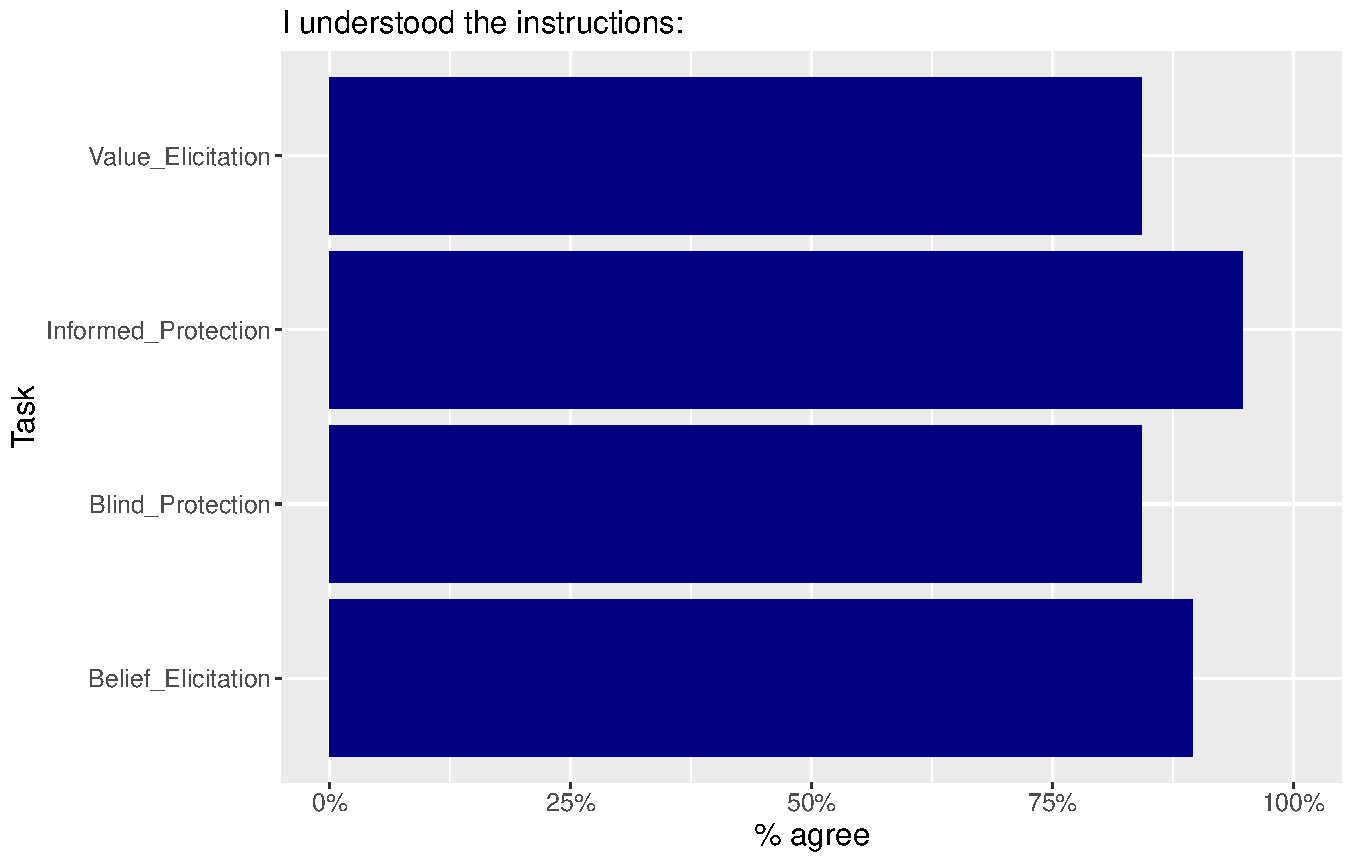
\includegraphics[width=\textwidth]{Graphs/Uplot1.pdf}
\end{subfigure}

\begin{subfigure}{0.6\textwidth}
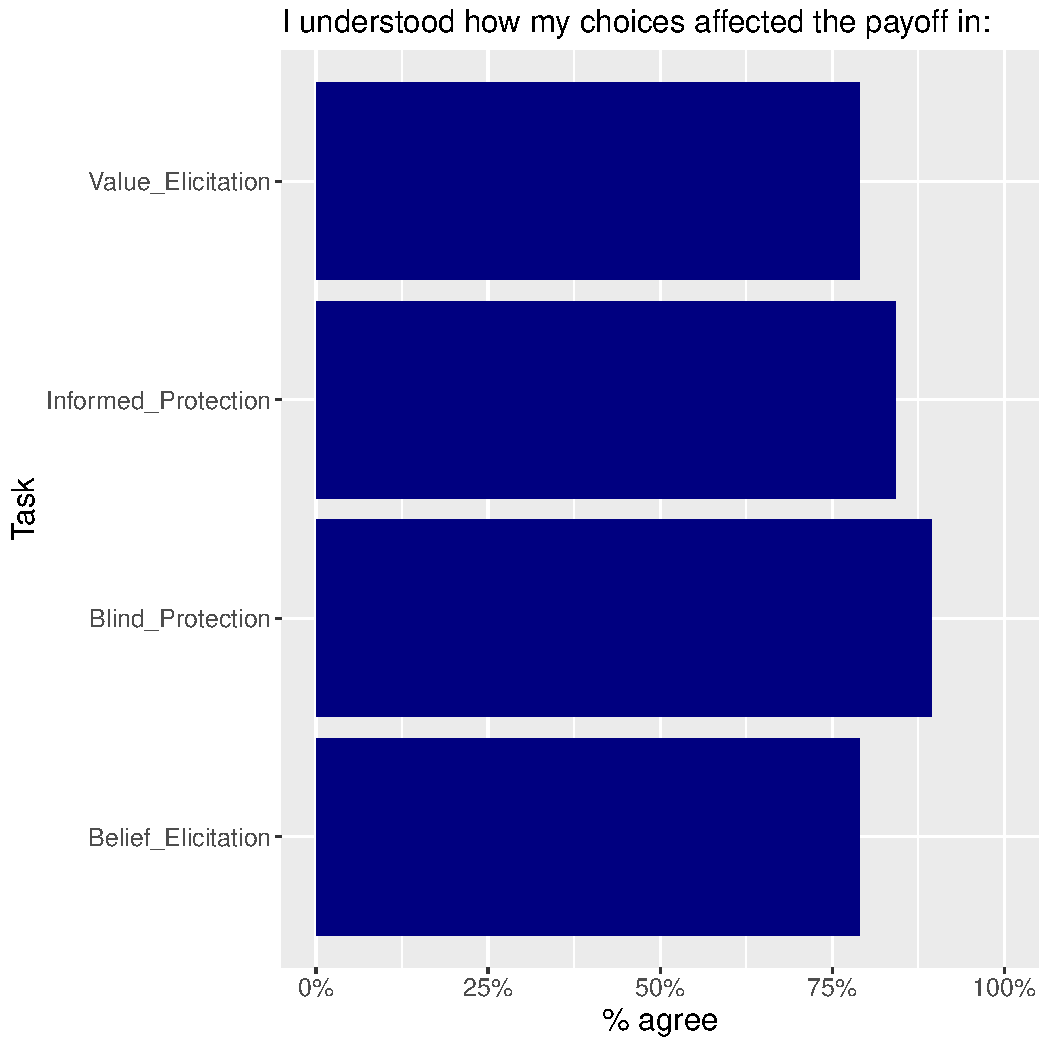
\includegraphics[width=\textwidth]{Graphs/Uplot2.pdf}
\end{subfigure}
\end{figure}
\end{frame}


\begin{frame}
\frametitle{Quiz answers correct}
\begin{itemize}
\item Most respondents make 1-3 mistakes out of 9 questions
\end{itemize}
\begin{figure}[h]
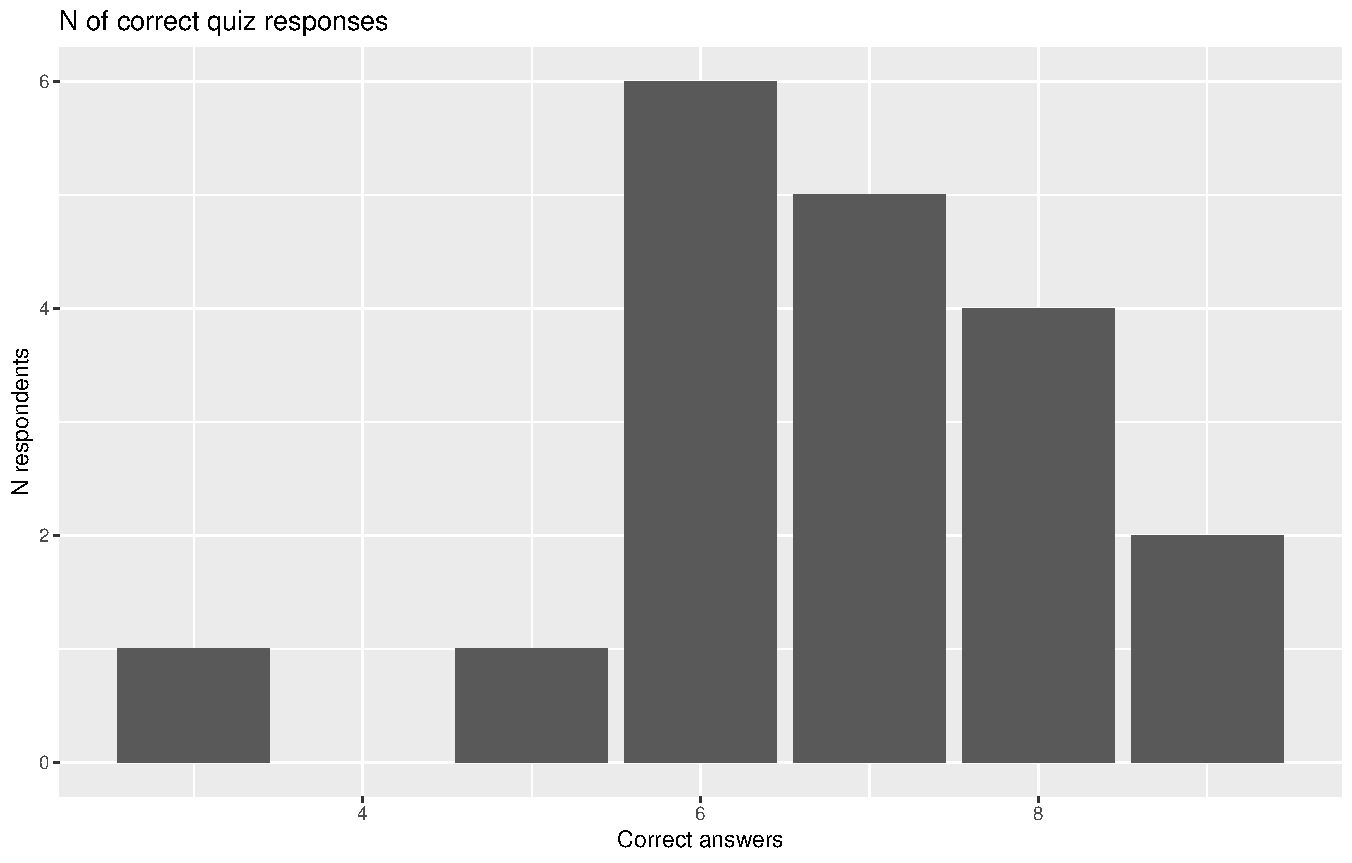
\includegraphics[scale=0.4]{Graphs/COMPRplot.pdf}
\end{figure}
\end{frame}





\begin{frame}
\frametitle{Uninformed Protection}
\begin{itemize}
\item There is more protection when the probability of black ball is higher
\item Noisy
\end{itemize}
\begin{figure}[h]
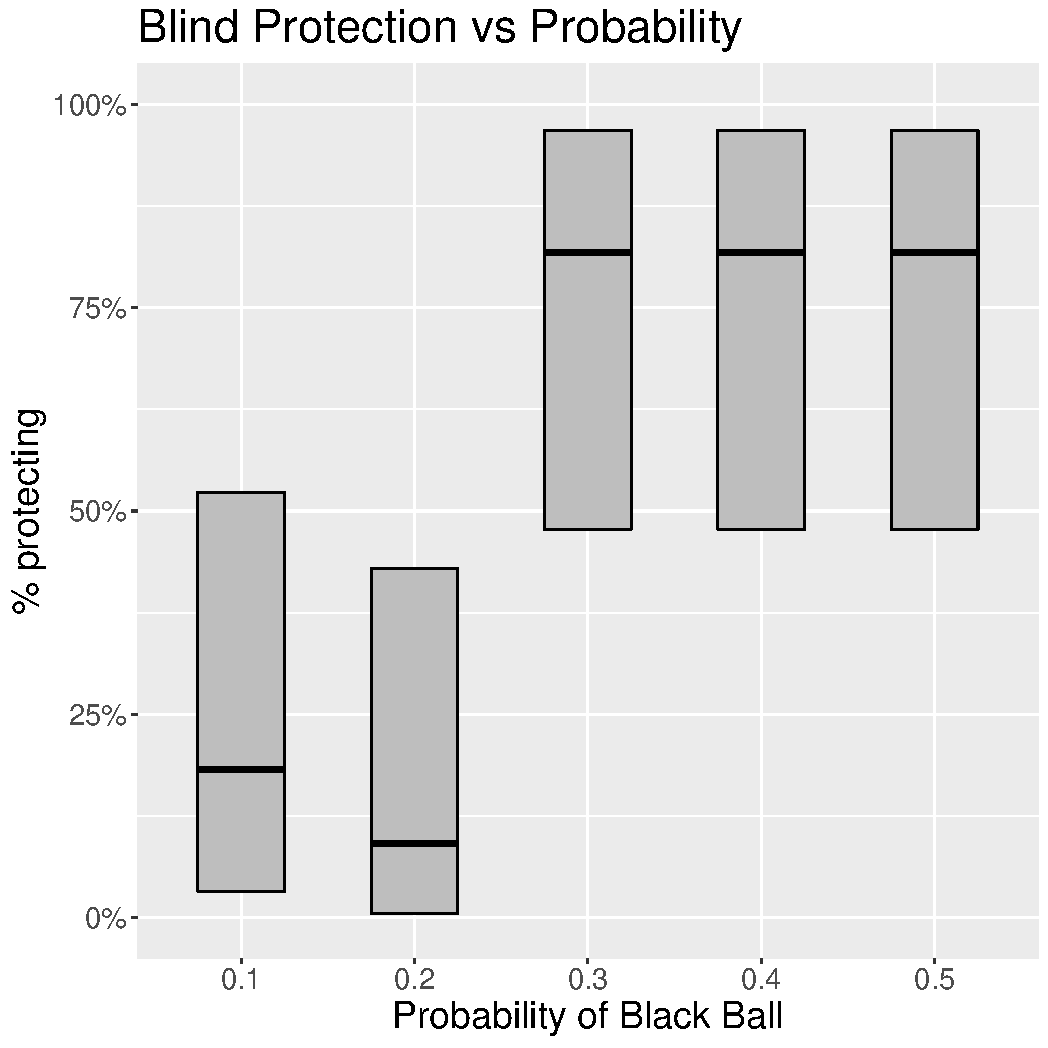
\includegraphics[scale=0.4]{Graphs/BLProt_plot2.pdf}
\end{figure}
\end{frame}




\begin{frame}
\frametitle{Informed Protection}
\begin{itemize}
\item There is more protection when the posterior probability of black ball is higher
\item Even more noisy, but hopefully corrected with larger sample
\item Need to check individual responses (fixed effects)
\end{itemize}
\begin{figure}[h]
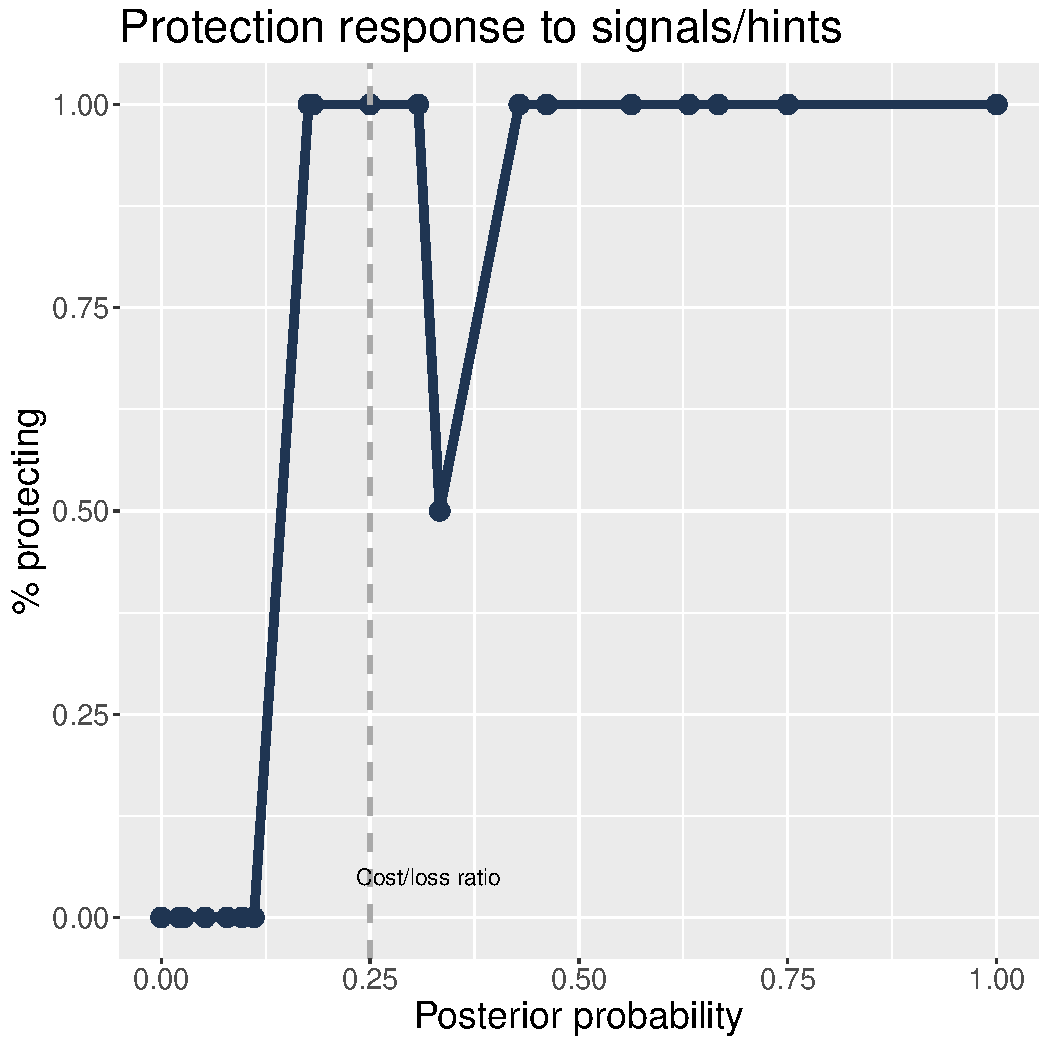
\includegraphics[scale=0.35]{Graphs/IP_plot.pdf}
\end{figure}
\end{frame}


\begin{frame}
\frametitle{Informed Protection: Correlation}
\footnotesize
\begin{table}[htbp]\centering
\def\sym#1{\ifmmode^{#1}\else\(^{#1}\)\fi}
\caption{Informed Protection}
\begin{tabular}{l*{4}{c}}
\hline\hline
                &\multicolumn{1}{c}{(1)}&\multicolumn{1}{c}{(2)}&\multicolumn{1}{c}{(3)}&\multicolumn{1}{c}{(4)}\\
                &\multicolumn{1}{c}{All}&\multicolumn{1}{c}{All}&\multicolumn{1}{c}{Smart}&\multicolumn{1}{c}{Smart}\\
\hline
Posterior prob. &     .663\sym{***}&     .114         &     .692\sym{***}&     .126         \\
                &    (8.5)         &    (0.9)         &    (9.4)         &    (0.8)         \\
Prior prob.     &                  &     .467\sym{***}&                  &     .519\sym{***}\\
                &                  &    (3.5)         &                  &    (3.1)         \\
Gremlin says Black&                  &     .497\sym{***}&                  &     .506\sym{***}\\
                &                  &    (5.8)         &                  &    (5.0)         \\
Constant        &     .235\sym{***}&    .0872\sym{**} &     .233\sym{***}&    .0678         \\
                &    (7.3)         &    (2.2)         &    (7.7)         &    (1.6)         \\
\hline
Observations    &      300         &      300         &      228         &      228         \\
Adjusted \(R^{2}\)&     0.35         &     0.41         &     0.36         &     0.42         \\
\hline\hline
\multicolumn{5}{l}{\footnotesize \textit{t} statistics in parentheses}\\
\multicolumn{5}{l}{\footnotesize \sym{*} \(p<0.10\), \sym{**} \(p<0.05\), \sym{***} \(p<0.01\)}\\
\end{tabular}
\end{table}


\end{frame}


\begin{frame}
\frametitle{Informed Protection: Determinants}
\footnotesize
\begin{table}[htbp]\centering
\def\sym#1{\ifmmode^{#1}\else\(^{#1}\)\fi}
\caption{Informed Protection: Response to Reported Beliefs}
\begin{tabular}{l*{3}{c}}
\hline\hline
                &\multicolumn{1}{c}{(1)}&\multicolumn{1}{c}{(2)}&\multicolumn{1}{c}{(3)}\\
                &\multicolumn{1}{c}{All}&\multicolumn{1}{c}{All}&\multicolumn{1}{c}{Smart}\\
\hline
Belief          &     .746\sym{***}&     .358\sym{**} &     .462\sym{**} \\
                &    (7.8)         &    (2.4)         &    (2.5)         \\
Posterior prob. &                  &     .424\sym{***}&     .367\sym{**} \\
                &                  &    (3.5)         &    (2.6)         \\
Constant        &     .206\sym{***}&     .189\sym{***}&     .178\sym{***}\\
                &    (5.3)         &    (4.8)         &    (4.6)         \\
\hline
Observations    &      300         &      300         &      228         \\
Adjusted \(R^{2}\)&     0.32         &     0.38         &     0.40         \\
\hline\hline
\multicolumn{4}{l}{\footnotesize \textit{t} statistics in parentheses}\\
\multicolumn{4}{l}{\footnotesize \sym{*} \(p<0.10\), \sym{**} \(p<0.05\), \sym{***} \(p<0.01\)}\\
\end{tabular}
\end{table}

\end{frame}


\begin{frame}
\frametitle{Informed Protection: Do Subject's Beliefs Matter?}
\footnotesize
\begin{table}[htbp]\centering
\def\sym#1{\ifmmode^{#1}\else\(^{#1}\)\fi}
\caption{Informed Protection: Response to Reported Beliefs}
\begin{tabular}{l*{3}{c}}
\hline\hline
                &\multicolumn{1}{c}{(1)}&\multicolumn{1}{c}{(2)}&\multicolumn{1}{c}{(3)}\\
                &\multicolumn{1}{c}{All}&\multicolumn{1}{c}{All}&\multicolumn{1}{c}{Smart}\\
\hline
Belief          &     .746\sym{***}&     .358\sym{**} &     .462\sym{**} \\
                &    (7.8)         &    (2.4)         &    (2.5)         \\
Posterior prob. &                  &     .424\sym{***}&     .367\sym{**} \\
                &                  &    (3.5)         &    (2.6)         \\
Constant        &     .206\sym{***}&     .189\sym{***}&     .178\sym{***}\\
                &    (5.3)         &    (4.8)         &    (4.6)         \\
\hline
Observations    &      300         &      300         &      228         \\
Adjusted \(R^{2}\)&     0.32         &     0.38         &     0.40         \\
\hline\hline
\multicolumn{4}{l}{\footnotesize \textit{t} statistics in parentheses}\\
\multicolumn{4}{l}{\footnotesize \sym{*} \(p<0.10\), \sym{**} \(p<0.05\), \sym{***} \(p<0.01\)}\\
\end{tabular}
\end{table}

\end{frame}



\begin{frame}
\frametitle{Belief Updating}
\begin{itemize}
\item A bit more correlation with actual posterior probabilities!
\item Even more if we exclude everybody scoring less than 7 out of 9 quiz questions
\end{itemize}
\begin{figure}[h]
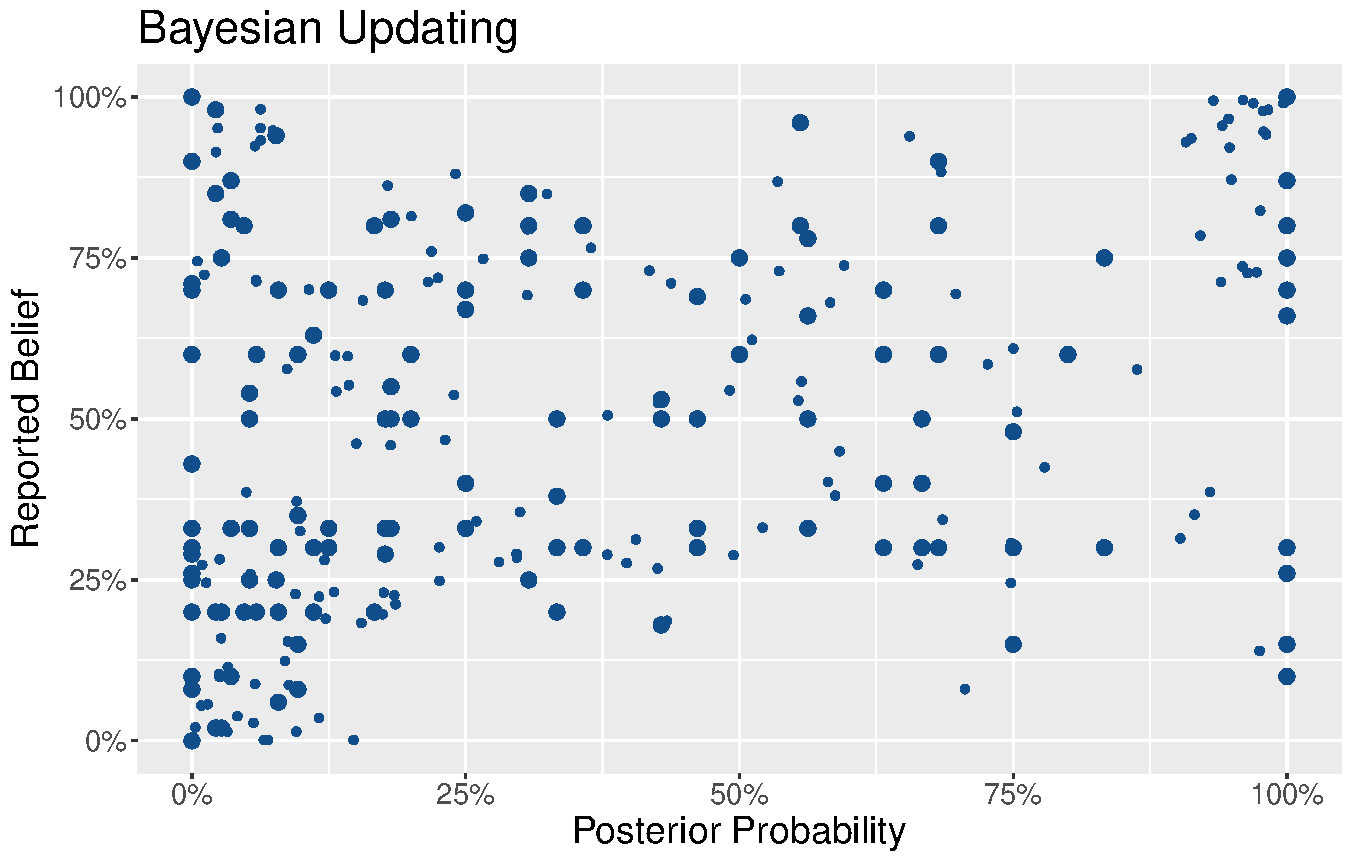
\includegraphics[scale=0.4]{Graphs/UPD_curve2.pdf}
\end{figure}
\end{frame}


\begin{frame}
\frametitle{Belief Updating: Correlation}
\footnotesize
\begin{table}[htbp]\centering
\def\sym#1{\ifmmode^{#1}\else\(^{#1}\)\fi}
\caption{Belief Elicitation: Belief vs Posterior}
\begin{tabular}{l*{3}{c}}
\hline\hline
                &\multicolumn{1}{c}{(1)}&\multicolumn{1}{c}{(2)}&\multicolumn{1}{c}{(3)}\\
                &\multicolumn{1}{c}{All}&\multicolumn{1}{c}{Not\_honest}&\multicolumn{1}{c}{Good quiz}\\
\hline
Posterior prob. &     .669\sym{***}&     .711\sym{***}&     .523\sym{***}\\
                &   (29.0)         &   (29.1)         &   (15.7)         \\
Constant        &     .151\sym{***}&     .147\sym{***}&     .226\sym{***}\\
                &   (16.2)         &   (14.1)         &   (17.8)         \\
\hline
Observations    &      780         &      636         &      520         \\
Adjusted \(R^{2}\)&     0.57         &     0.61         &     0.39         \\
\hline\hline
\multicolumn{4}{l}{\footnotesize \textit{t} statistics in parentheses}\\
\multicolumn{4}{l}{\footnotesize \sym{*} \(p<0.10\), \sym{**} \(p<0.05\), \sym{***} \(p<0.01\)}\\
\end{tabular}
\end{table}


\end{frame}

\begin{frame}
\frametitle{What Affects Beliefs?}
\footnotesize
\begin{table}[htbp]\centering
\def\sym#1{\ifmmode^{#1}\else\(^{#1}\)\fi}
\caption{Belief Elicitation: Discrepancy}
\begin{tabular}{l*{6}{c}}
\hline\hline
                &\multicolumn{1}{c}{(1)}&\multicolumn{1}{c}{(2)}&\multicolumn{1}{c}{(3)}&\multicolumn{1}{c}{(4)}&\multicolumn{1}{c}{(5)}&\multicolumn{1}{c}{(6)}\\
                &\multicolumn{1}{c}{}&\multicolumn{1}{c}{}&\multicolumn{1}{c}{}&\multicolumn{1}{c}{}&\multicolumn{1}{c}{}&\multicolumn{1}{c}{}\\
\hline
FN rate         &     .016         &     .016         &    -.014         &    -.014         &   -.0562         &   -.0554         \\
                &    (0.1)         &    (0.1)         &    (0.1)         &    (0.1)         &    (0.1)         &    (0.1)         \\
FP rate         &     .919\sym{***}&     .919\sym{***}&     1.07\sym{***}&     1.07\sym{***}&     1.05\sym{***}&     1.05\sym{***}\\
                &    (0.1)         &    (0.1)         &    (0.1)         &    (0.1)         &    (0.1)         &    (0.1)         \\
Good quiz       &                  &                  &    .0469         &    .0673         &                  &                  \\
                &                  &                  &    (0.0)         &    (0.0)         &                  &                  \\
Good quiz $\times$ FN rate&                  &                  &    .0463         &    .0464         &                  &                  \\
                &                  &                  &    (0.1)         &    (0.1)         &                  &                  \\
Good quiz $\times$ FP rate&                  &                  &    -.286\sym{*}  &    -.284\sym{*}  &                  &                  \\
                &                  &                  &    (0.2)         &    (0.2)         &                  &                  \\
Stat. class     &                  &                  &                  &                  &  -.00193         &   -.0127         \\
                &                  &                  &                  &                  &    (0.0)         &    (0.0)         \\
Stat. class $\times$ FN rate&                  &                  &                  &                  &     .127         &     .126         \\
                &                  &                  &                  &                  &    (0.1)         &    (0.1)         \\
Stat. class $\times$ FP rate&                  &                  &                  &                  &    -.229         &    -.226         \\
                &                  &                  &                  &                  &    (0.2)         &    (0.2)         \\
Constant        &    -.076\sym{***}&   -.0656\sym{***}&    -.101\sym{***}&    -.102\sym{***}&   -.0751\sym{***}&   -.0563         \\
                &    (0.0)         &    (0.0)         &    (0.0)         &    (0.0)         &    (0.0)         &    (0.0)         \\
Prior prob dummies &       No         &      Yes         &       No         &      Yes         &       No         &      Yes         \\
\hline
Observations    &      630         &      630         &      630         &      630         &      630         &      630         \\
Adjusted \(R^{2}\)&     0.17         &     0.17         &     0.17         &     0.17         &     0.17         &     0.17         \\
\hline\hline
\multicolumn{7}{l}{\footnotesize Standard errors in parentheses}\\
\multicolumn{7}{l}{\footnotesize \sym{*} \(p<0.10\), \sym{**} \(p<0.05\), \sym{***} \(p<0.01\)}\\
\end{tabular}
\end{table}

\end{frame}


\begin{frame}
\frametitle{Belief Updating: Decomposition}
\footnotesize
\begin{table}[htbp]\centering
\def\sym#1{\ifmmode^{#1}\else\(^{#1}\)\fi}
\caption{Belief Elicitation: Decomposition}
\begin{tabular}{l*{3}{c}}
\hline\hline
                &\multicolumn{1}{c}{(1)}&\multicolumn{1}{c}{(2)}&\multicolumn{1}{c}{(3)}\\
                &\multicolumn{1}{c}{OLS}&\multicolumn{1}{c}{FE}&\multicolumn{1}{c}{Smart, FE}\\
\hline
lt\_prior        &     .178         &     .205\sym{**} &     .231\sym{**} \\
                &    (1.4)         &    (2.5)         &    (2.2)         \\
signalB         &   -.0835         &     .735\sym{**} &     .988\sym{**} \\
                &   (-0.2)         &    (2.5)         &    (2.5)         \\
signalW         &     .818\sym{***}&        0         &        0         \\
                &    (2.8)         &      (.)         &      (.)         \\
Constant        &     .332         &    -.471\sym{**} &    -.577\sym{**} \\
                &    (0.9)         &   (-2.7)         &   (-2.6)         \\
\hline
Observations    &       68         &       68         &       52         \\
Adjusted \(R^{2}\)&     0.16         &     0.20         &     0.25         \\
\hline\hline
\multicolumn{4}{l}{\footnotesize \textit{t} statistics in parentheses}\\
\multicolumn{4}{l}{\footnotesize \sym{*} \(p<0.10\), \sym{**} \(p<0.05\), \sym{***} \(p<0.01\)}\\
\end{tabular}
\end{table}

\end{frame}


\begin{frame}
\frametitle{WTP for signals}
\begin{itemize}
\item Higher average WTP for more valuable signals
\item Within-analysis pending
\end{itemize}
\begin{figure}[h]
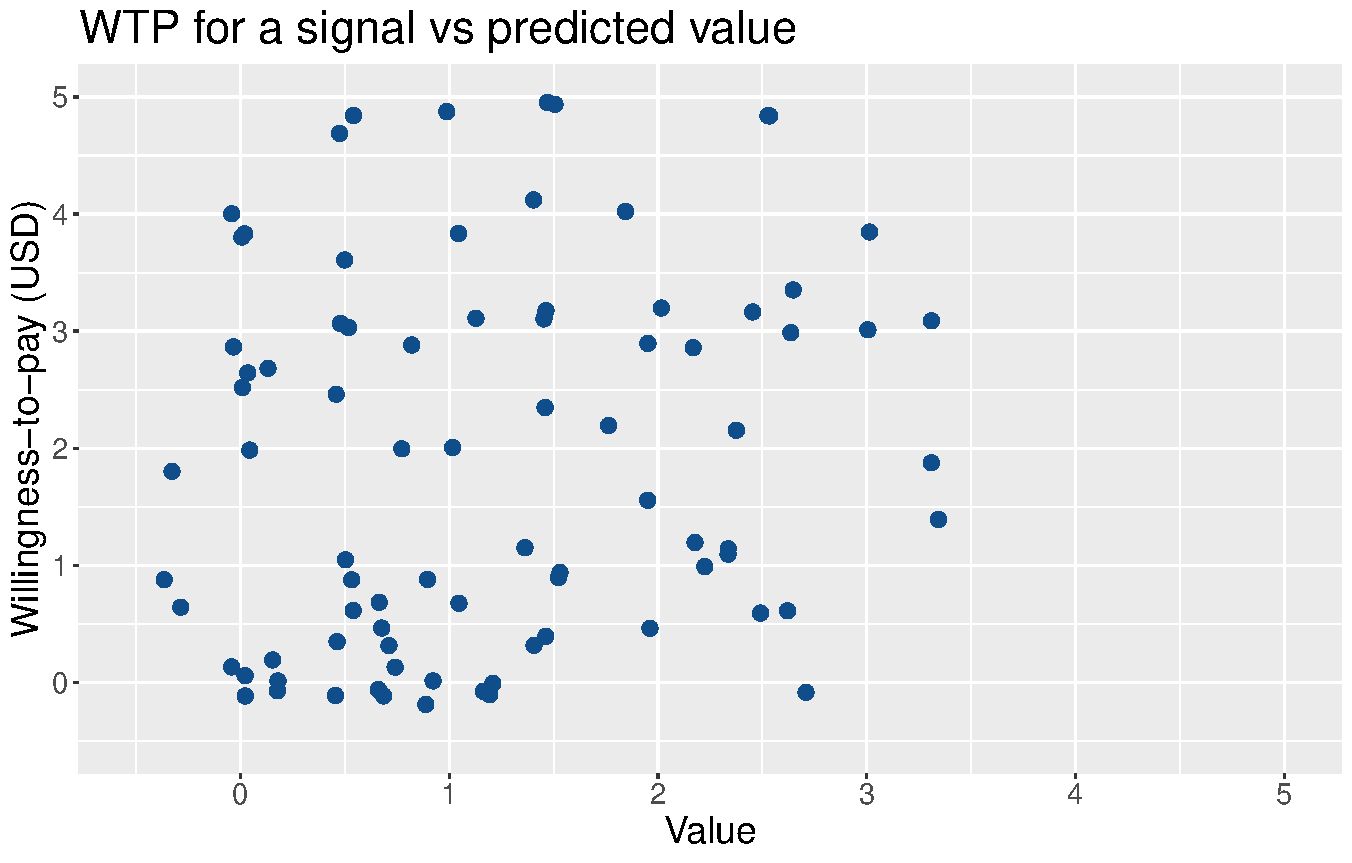
\includegraphics[scale=0.4]{Graphs/WTP_curve2.pdf}
\end{figure}
\end{frame}

\begin{frame}
\frametitle{WTP for signals: Determinants}
\footnotesize
\begin{table}[htbp]\centering
\def\sym#1{\ifmmode^{#1}\else\(^{#1}\)\fi}
\caption{WTP for Information}
\begin{tabular}{l*{5}{c}}
\hline\hline
                &\multicolumn{1}{c}{(1)}&\multicolumn{1}{c}{(2)}&\multicolumn{1}{c}{(3)}&\multicolumn{1}{c}{(4)}&\multicolumn{1}{c}{(5)}\\
                &\multicolumn{1}{c}{OLS}&\multicolumn{1}{c}{OLS}&\multicolumn{1}{c}{FE}&\multicolumn{1}{c}{FE}&\multicolumn{1}{c}{FE}\\
\hline
value           &     .688\sym{***}&      .71\sym{***}&     .713\sym{***}&     .381\sym{***}&     .135         \\
                &    (5.1)         &    (5.5)         &    (5.4)         &    (3.4)         &    (1.3)         \\
(sum) bp        &                  &    -.452\sym{***}&                  &                  &                  \\
                &                  &   (-4.3)         &                  &                  &                  \\
honest\_treatment&                  &                  &                  &     1.26\sym{***}&    -.248         \\
                &                  &                  &                  &    (3.1)         &   (-0.4)         \\
False neg. rate &                  &                  &                  &                  &    -3.94\sym{***}\\
                &                  &                  &                  &                  &   (-3.5)         \\
False pos. rate &                  &                  &                  &                  &    -6.08\sym{***}\\
                &                  &                  &                  &                  &   (-3.3)         \\
Constant        &     .961\sym{***}&     2.11\sym{***}&     .918\sym{***}&     1.07\sym{***}&     3.21\sym{***}\\
                &    (4.0)         &    (5.5)         &    (4.1)         &    (5.6)         &    (6.6)         \\
\hline
Observations    &      114         &      114         &      114         &      114         &      114         \\
Adjusted \(R^{2}\)&     0.18         &     0.25         &     0.29         &     0.41         &     0.53         \\
\hline\hline
\multicolumn{6}{l}{\footnotesize \textit{t} statistics in parentheses}\\
\multicolumn{6}{l}{\footnotesize \sym{*} \(p<0.10\), \sym{**} \(p<0.05\), \sym{***} \(p<0.01\)}\\
\end{tabular}
\end{table}


\end{frame}

\end{document}
